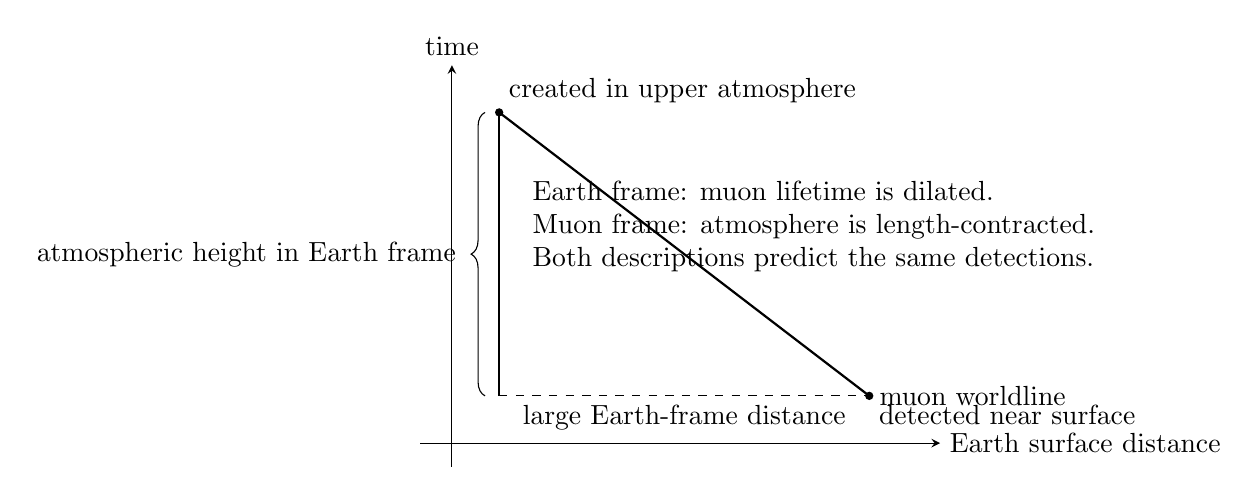
\begin{tikzpicture}[x=1cm,y=1cm,>=stealth]
    \draw[->] (-0.4,0) -- (6.2,0) node[right] {Earth surface distance};
    \draw[->] (0,-0.3) -- (0,4.8) node[above] {time};

    \draw[thick] (0.6,4.2) -- (5.3,0.6) node[right] {muon worldline};
    \fill (0.6,4.2) circle (1.5pt) node[above right] {created in upper atmosphere};
    \fill (5.3,0.6) circle (1.5pt) node[below right] {detected near surface};

    \draw[thick] (0.6,4.2) -- (0.6,0.6);
    \draw[decorate,decoration={brace,amplitude=5pt}] (0.42,0.6) -- (0.42,4.2)
    node[midway,left=7pt] {atmospheric height in Earth frame};

    \draw[dashed] (0.6,0.6) -- (5.3,0.6);
    \node[below] at (2.95,0.6) {large Earth-frame distance};

    \node[align=left,anchor=west] at (0.9,2.75)
    {Earth frame: muon lifetime is dilated.\\Muon frame: atmosphere is length-contracted.\\Both descriptions predict the same detections.};
\end{tikzpicture}
